\section{Information Theorethic Learning on Autoencoders}

The Information Theorethic Learning concept was introduced in \cite{Principe_2000} to extend the Mean-Square error criterion to cost functions including information about the training data. The goal was to manipulate the information being carried in the data or, in other words, to find cost functions that would be able to directly influence information. The name ITL is a natural transition from the aforementioned proccess, as the machine learning function had to be independent from the informational transition of data. \par

The Autoencoder was first proposed to test the concepts of ITL on \cite{Santana_2016}. Using similar theoretic descriptors as the Entropy Triangle, like Mutual Information and entropy, the work of the researchers consists of trying to prove the validity of their theories by using the Autoencoder. Particularly, they are looking at the representation of the $\hat{Z}$ and the reconstructed value of $\overline{X}$ to calculate the loss function.

\begin{equation}\label{eq:Principe_loss_function}
cost = L(x,\overline{X}) + \lambda \times R(E,P)
\end{equation}

On Equation \ref{eq:Principe_loss_function} $L$ is the reconstruction cost function measuring the loss between the original $X$ and the predicted $\overline{X}$ at the output of the Autoencoder. $R$ is a functional regularization that uses information theoretic measures.\par

\begin{figure}[H]
	\centering	
	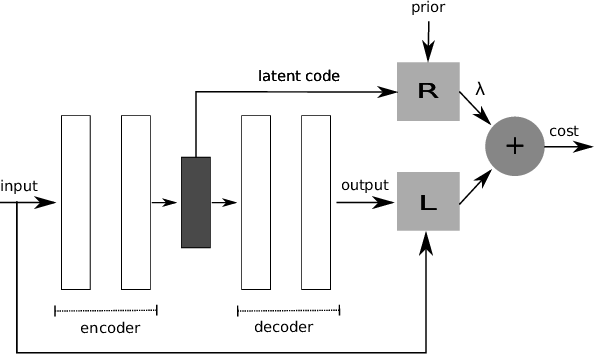
\includegraphics[width=\linewidth]{Principe_Autoencoder}
	\caption{Autoencoder illustrating Equation \ref{eq:Principe_loss_function} from \cite{Santana_2016}.}
	\label{fig:figure_autoencoder}
\end{figure} 

On \cite{Yu_2019} Principe and Yu expand on the use of Autoencoders and explore some of its key aspects regarding the bottleneck layer. By analyzing the remarkable similarities between a transmission channel and the Autocoder(an structure also proposed in this report) they use widespread available materials and datasets to evaluate the capacity of a stacked Autoencoder (as we do on our experiments) to demonstrate the ITL. 

